%! Author = Omar Iskandarani
%! Date = 1/26/2026
%! Affiliation = Independent Researcher, Groningen, The Netherlands
%! License = © 2025 Omar Iskandarani. All rights reserved. This manuscript is made available for academic reading and citation only. No republication, redistribution, or derivative works are permitted without explicit written permission from the author. Contact: info@omariskandarani.com
%! ORCID = 0009-0006-1686-3961
%! DOI = 10.5281/zenodo.xxx

\newcommand{\paperdoi}{10.5281/zenodo.18388706}
\newcommand{\papertitle}{Helicity-Constrained Stability Beyond Energy Minimization}

%=========================================
% % PREAMBLE, PACKAGES AND DOCUMENT CONFIGURATION
%=========================================
\documentclass[11pt]{article}
\usepackage{amsmath,amssymb,amsfonts,bm}
\usepackage{siunitx}
\usepackage[hidelinks]{hyperref}
\usepackage[a4paper,margin=1in]{geometry}
\usepackage[T1]{fontenc}
\usepackage[utf8]{inputenc}
\usepackage{tikz}

% swirl arrows (context-aware)
\newcommand{\swirlarrow}{\mkern-2mu\scriptscriptstyle\boldsymbol{\circlearrowleft}}
\newcommand{\vswirl}{\mathbf{v}_{\mkern-2mu\scriptscriptstyle\boldsymbol{\circlearrowleft}}}
\newcommand{\SwirlClock}{S_{(t)}^{\mkern-2mu\scriptscriptstyle\boldsymbol{\circlearrowleft}}}
\newcommand{\Fmaxswirl}{F^{\max}_{\mkern-1mu\scriptscriptstyle\boldsymbol{\circlearrowleft}}}
\newcommand{\Fmax}{F^{\max}_{\mkern-1mu\scriptscriptstyle\boldsymbol{\circlearrowleft}}} 
\newcommand{\FmaxEM}{F^{\max}_{\mathrm{EM}}}
\newcommand{\FmaxG}{F_{\mathrm{G}}^{\max}}               % G-like maximal force scale
\newcommand{\vscore}{v_{\swirlarrow}}                    % shorthand: |v_swirl| at r=r_c
\newcommand{\vnorm}{\lVert \mathbf{v}_{\mkern-2mu\scriptscriptstyle\boldsymbol{\circlearrowleft}} \rVert}  %swirl speed magnitude
\newcommand{\rhoF}{\rho_{\!f}}\newcommand{\rhof}{\rho_{\!f}}     % effective fluid density
\newcommand{\rhoE}{\rho_{\!E}}\newcommand{\rhoe}{\rho_{\!E}}                           % swirl energy density
\newcommand{\rhoM}{\rho_{\!m}}\newcommand{\rhom}{\rho_{\!m}}                           % mass-equivalent density
\newcommand{\omegas}{\boldsymbol{\omega}_{\swirlarrow}}  % swirl vorticity
\newcommand{\Om}{\Omega_{\swirlarrow}}                   % swirl angular frequency profile
\newcommand{\rc}{r_c}                                    % string core radius (swirl string radius)


\newcommand{\titlepageOpen}{
    \begin{titlepage}
        \thispagestyle{empty}  \centering
        \Large \bfseries \papertitle \par \vspace{1cm}
        {\Large \itshape \textbf{Omar Iskandarani}\textsuperscript{\textbf{*}} \par} \vspace{0.5cm}
        {\today \par}  \vspace{0.5cm}
}

\newcommand{\titlepageClose}{
        \vfill \raggedright \null
        \begin{picture}(0,0)
            \put(0,-45){  % Shift 200pt left, 40pt down
                \begin{minipage}[b]{0.7\textwidth} \footnotesize
                    \renewcommand{\arraystretch}{1.0} \noindent\rule{\textwidth}{0.4pt} \\[0.5em]
                    \textsuperscript{\textbf{*}} Independent Researcher, Groningen, The Netherlands \\
                    Email: \texttt{info@omariskandarani.com} \\
                    ORCID: \texttt{\href{https://orcid.org/0009-0006-1686-3961}{0009-0006-1686-3961}} \\
                    DOI: \href{https://doi.org/\paperdoi}{\paperdoi}
                \end{minipage}
            }
        \end{picture}
    \end{titlepage}
}
%=========================================
% Start Document - Title Page
%=========================================
\begin{document}
    \titlepageOpen
        \begin{abstract}
            Stability in classical continuum systems is commonly associated with energetic
            optimality, whereby persistent configurations correspond to minima of an
            appropriate energy functional. However, ideal incompressible flows admit
            long-lived localized structures that do not satisfy this criterion. In
            particular, knotted vortex filaments have been observed to persist for many
            characteristic times despite not corresponding to energy-minimizing states.

            In this work, we show that the longevity of knotted vortex filaments in ideal
            incompressible flows arises from topological constraints imposed by helicity
            conservation, rather than energetic optimality. By analyzing helicity as an
            active dynamical constraint, we demonstrate that conserved topological
            invariants restrict admissible decay pathways and obstruct continuous
            transitions between distinct topological classes. As a result, knotted
            configurations remain stable in the sense of long-term persistence, even while
            undergoing continuous dynamical evolution.

            We distinguish energetic stability from topological stability and show that the
            latter provides an independent mechanism for robustness in classical continuum
            systems. Knotted vortex filaments exemplify this mechanism, persisting far from
            energetic equilibrium due to the structure of the admissible configuration
            space defined by the Euler equations. These results clarify the role of topology
            in classical fluid dynamics and suggest that conserved topological quantities
            should be regarded as fundamental contributors to stability, robustness, and
            structure formation in ideal and near-ideal flows.
        \end{abstract}
    \titlepageClose

%==============================================================================
% SST-61_Topological_Stabilization_Ideal_Flows.tex
%==============================================================================

    \section{Introduction}

        Stability in classical continuum systems is commonly associated with energetic
        optimality: configurations persist because they minimize an appropriate energy
        functional subject to external constraints. This paradigm underlies much of
        classical mechanics, elasticity, and fluid dynamics \cite{arnold1966,landau_fluid}. However, a growing body of
        evidence from ideal fluid flows, plasmas, and related systems indicates the
        existence of long-lived localized structures that do not correspond to global
        energy minima, yet remain dynamically stable over extended timescales.

        In inviscid, incompressible flows, vortex filaments can form closed and knotted
        configurations that propagate, deform, and interact without rapid decay.
        Experimental and numerical studies have demonstrated that such knotted
        structures may persist for many turnover times, even in the absence of
        confinement or external forcing.
        \cite{kleckner2013,scheeler2014}.
        Their longevity cannot be explained solely by
        energetic considerations, as these configurations are generally not stationary
        solutions of minimal energy.

        Ideal fluid dynamics possesses conserved quantities that go beyond energy and
        momentum. Among these, helicity plays a distinguished role as a global invariant
        that encodes the topological structure of the flow.
        \cite{moffatt1969}.
        While helicity has
        traditionally been employed as a diagnostic measure of knottedness or linkage,
        its role as an active constraint on the dynamics has received comparatively less
        attention.

        In this work, we show that helicity conservation imposes topological constraints
        that stabilize localized knotted structures independently of energetic
        optimality. We argue that the persistence of such structures is best understood
        as a consequence of topological obstruction to decay, rather than proximity to
        an energy minimum. This perspective provides a unified explanation for the
        observed longevity of knotted vortex filaments and clarifies the distinction
        between energetic and topological stability in ideal continuum systems.

        ---

    \section{Ideal Flow Framework and Helicity Conservation}

        We consider a three-dimensional, incompressible, inviscid fluid described by the
        Euler equations,
        \begin{equation}
            \partial_t \mathbf{v} + (\mathbf{v}\cdot\nabla)\mathbf{v}
            = -\nabla p,
            \qquad
            \nabla\cdot\mathbf{v} = 0,
        \end{equation}
        where $\mathbf{v}(\mathbf{x},t)$ is the velocity field and $p$ is the pressure
        enforcing incompressibility. We assume the flow to be barotropic and free of
        external forcing and dissipation.

        Under these conditions, Kelvin's circulation theorem guarantees the conservation
        of circulation along material loops advected by the flow.
        \cite{kelvin1869}.
        A direct consequence
        is the conservation of helicity,
        \begin{equation}
            H = \int_V \mathbf{v}\cdot(\nabla\times\mathbf{v})\,\mathrm{d}V,
        \end{equation}
        provided the velocity field remains smooth and reconnection events are absent.

        Helicity is a pseudoscalar quantity that measures the degree of linkage between
        vortex lines.
        \cite{moffatt1969,ricca1996}.
        Unlike energy, which is sensitive to local deformation, helicity
        is invariant under continuous deformations of the flow that preserve topology.
        As such, it encodes global structural information that cannot be altered by
        smooth dynamics alone.

        In many treatments, helicity is regarded as a passive invariant, useful for
        characterizing flow complexity or diagnosing turbulent cascades. Here, we
        instead emphasize its role as a dynamical constraint: helicity conservation
        restricts the class of admissible flow evolutions and forbids continuous decay
        pathways that would alter the topological structure of vortex filaments.

        ---


    \section{Helicity as a Topological Constraint}

        For flows dominated by thin vortex filaments with circulations $\Gamma_i$,
        helicity admits a decomposition into topological contributions,
        \begin{equation}
            H = \sum_{i\neq j} \Gamma_i \Gamma_j\, \mathrm{Lk}_{ij}
            + \sum_i \Gamma_i^2(\mathrm{Tw}_i + \mathrm{Wr}_i),
        \end{equation}
        where $\mathrm{Lk}_{ij}$ denotes the Gauss linking number between filaments $i$
        and $j$, while $\mathrm{Tw}_i$ and $\mathrm{Wr}_i$ represent the twist and writhe
        of filament $i$, respectively.

        This decomposition makes explicit that helicity is fundamentally topological in
        nature. The linking numbers are integer-valued invariants, unchanged under smooth
        deformations of the flow, while twist and writhe may interchange continuously so
        long as their sum remains fixed. As a result, the total helicity is conserved
        even as individual geometric features evolve.

        \begin{figure}[t]
            \centering
            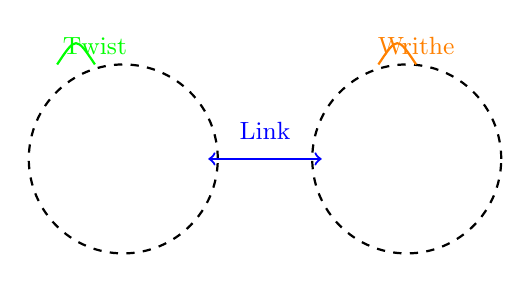
\begin{tikzpicture}[scale=1.2, thick]
                % Two dashed loops
                \draw[dashed] (1.5,1.5) circle (1);
                \draw[dashed] (4.5,1.5) circle (1);

                % Linking arrow
                \draw[<->, blue, thick] (2.4,1.5) -- (3.6,1.5);
                \node[blue] at (3,1.8) {\small Link};

                % Twist (helix symbol on left loop)
                \draw[green, thick] (0.8,2.5) .. controls (1,2.8) .. (1.2,2.5);
                \node[green] at (1.2,2.7) {\small Twist};

                % Writhe (wave on right loop)
                \draw[orange, thick] (4.2,2.5) .. controls (4.4,2.8) .. (4.6,2.5);
                \node[orange] at (4.6,2.7) {\small Writhe};
            \end{tikzpicture}

            \caption{
                Schematic illustration of helicity decomposition in a vortex filament.
                Helicity receives contributions from pairwise linking between filaments
                (\emph{link}), as well as internal geometric structure of individual filaments
                through \emph{twist} and \emph{writhe}. Continuous deformations may redistribute
                twist and writhe while preserving total helicity, whereas changes in linking
                require reconnection or dissipation.
            }
            \label{fig:helicity_decomposition}
        \end{figure}

        The key implication is that knotted or linked vortex configurations cannot be
        continuously transformed into unknotted states without violating helicity
        conservation. Any decay process that would eliminate knotting necessarily
        requires either reconnection or dissipation, both of which lie outside the
        ideal-flow framework.

        We therefore interpret helicity not merely as a measure of flow complexity, but
        as a topological constraint that actively restricts admissible dynamical
        evolutions. In particular, helicity conservation obstructs decay pathways that
        would otherwise lead to topologically simpler configurations.


    \section{Knotted Structures as Long-Lived Localized Excitations}

        Closed vortex filaments in ideal incompressible flows admit a wide range of
        topological configurations, including linked and knotted states. Experimental
        visualizations and numerical simulations have shown that such structures can
        propagate, deform, and interact over extended timescales while preserving their
        topological identity. In contrast to unknotted vortex rings, which may readily
        expand or relax through smooth deformations, knotted filaments exhibit a marked
        resistance to topological simplification.

        A defining characteristic of knotted vortex configurations is the localization
        of kinetic energy along the filament core. Although the induced velocity field
        extends throughout the surrounding fluid, the dominant energetic contribution
        remains concentrated within a narrow tubular region. This localization persists
        in the absence of boundaries, external confinement, or imposed potentials, and
        is maintained solely by the internal structure of the flow.

        \begin{figure}[t]
            \centering
            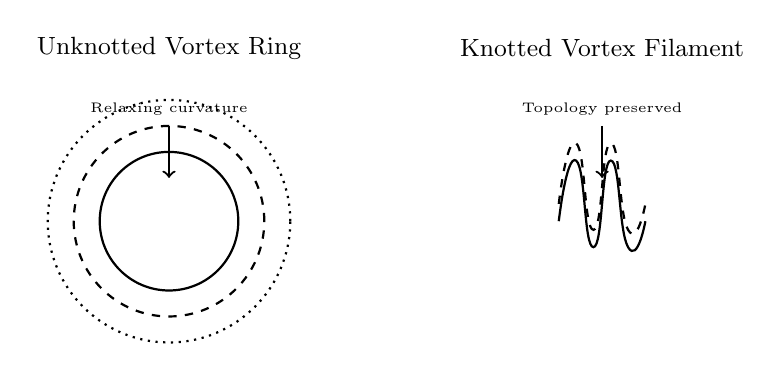
\begin{tikzpicture}[scale=1.1, thick]
                % Unknotted (Left)
                \node at (1.5, 3.5) {\small Unknotted Vortex Ring};

                \draw[dashed] (1.5,1.5) circle (1.1);
                \draw[dotted] (1.5,1.5) circle (1.4);
                \draw (1.5,1.5) circle (0.8);
                \draw[->] (1.5,2.6) -- (1.5,2);

                \node at (1.5,2.8) {\tiny Relaxing curvature};

                % Knotted (Right)
                \node at (6.5, 3.5) {\small Knotted Vortex Filament};

                \draw[black, thick] plot[smooth,tension=1] coordinates {(6,1.5) (6.2,2.2) (6.4,1.2) (6.6,2.2) (6.8,1.2) (7,1.5)};
                \draw[black, dashed] plot[smooth,tension=1] coordinates {(6,1.7) (6.2,2.4) (6.4,1.4) (6.6,2.4) (6.8,1.4) (7,1.7)};
                \draw[->] (6.5,2.6) -- (6.5,2);

                \node at (6.5,2.8) {\tiny Topology preserved};
            \end{tikzpicture}

            \caption{
                Comparison of the evolution of unknotted and knotted vortex filaments in an
                ideal incompressible flow. Unknotted vortex rings may deform continuously toward
                lower-curvature configurations, whereas knotted filaments preserve their
                topological structure over many characteristic times, exhibiting sustained
                energy localization.
            }
            \label{fig:knotted_vs_unknotted}
        \end{figure}

        The energetic properties of knotted filaments are constrained by their topology.
        For a filament of fixed circulation and core thickness, geometric knot theory
        implies the existence of lower bounds on filament length and curvature. These
        bounds translate into corresponding constraints on the kinetic energy, such that
        \begin{equation}
            E(K) \;\ge\; C\,\mathrm{Ropelength}(K),
        \end{equation}
        where $E(K)$ denotes the kinetic energy associated with a filament of knot type
        $K$, $\mathrm{Ropelength}(K)$ is the minimal length of a tube of fixed radius
        realizing that knot, and $C$ is a constant determined by the circulation and core
        structure. This inequality does not imply energetic optimality, but establishes
        that increased topological complexity carries an unavoidable energetic cost.

        Despite this, knotted vortex filaments are not observed to relax toward
        stationary energy minima. Instead, they persist in dynamically evolving states
        that continually redistribute curvature, twist, and writhe along the filament
        while preserving global topological invariants. Their longevity therefore cannot
        be attributed to energetic trapping in a potential well.

        \begin{figure}[t]
            \centering
            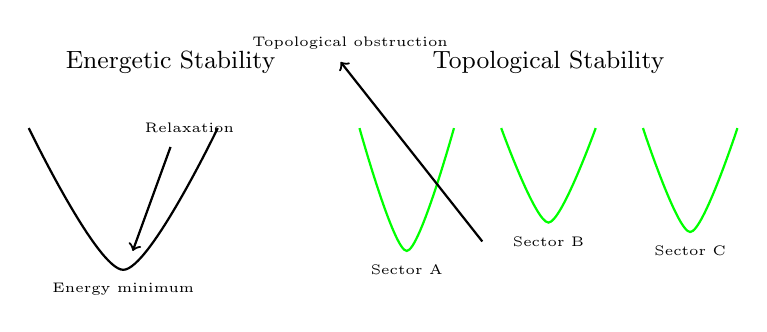
\begin{tikzpicture}[scale=1.2, thick]

                % Energetic Stability (Left)
                \node at (2, 3.2) {\small Energetic Stability};
                \draw[thick] plot[smooth] coordinates {(0.5,2.5) (1.5,1) (2.5,2.5)};
                \node at (1.5,0.8) {\tiny Energy minimum};
                \draw[->] (2,2.3) -- (1.6,1.2);
                \node at (2.2,2.5) {\tiny Relaxation};

                % Topological Stability (Right)
                \node at (6, 3.2) {\small Topological Stability};
                \draw[green, thick] plot[smooth] coordinates {(4,2.5) (4.5,1.2) (5,2.5)};
                \draw[green, thick] plot[smooth] coordinates {(5.5,2.5) (6,1.5) (6.5,2.5)};
                \draw[green, thick] plot[smooth] coordinates {(7,2.5) (7.5,1.4) (8,2.5)};
                \node at (4.5,1) {\tiny Sector A};
                \node at (6,1.3) {\tiny Sector B};
                \node at (7.5,1.2) {\tiny Sector C};

                \draw[->] (5.3,1.3) -- (3.8,3.2);
                \node at (3.9,3.4) {\tiny Topological obstruction};

            \end{tikzpicture}

            \caption{
                Schematic illustration of stability mechanisms in ideal flows. Energetic
                stability corresponds to relaxation toward minima of an energy functional,
                whereas topological stability arises from obstruction of admissible decay
                pathways by conserved invariants. Knotted vortex filaments exemplify the latter
                mechanism.
            }
            \label{fig:energy_vs_topology}
        \end{figure}

        For unknotted structures, continuous deformations may reduce curvature and
        energy without altering circulation. By contrast, any decay process that would
        eliminate knotting requires a change in topological invariants and is therefore
        forbidden within the ideal-flow framework. Reconnection or dissipation is
        necessary to bypass this obstruction.

        We therefore identify knotted vortex filaments as long-lived localized
        excitations whose persistence arises from topological obstruction rather than
        energetic stability. This distinction clarifies why such structures remain robust
        despite not corresponding to energy-minimizing configurations and motivates a
        reassessment of stability criteria in classical continuum systems.

    \section{Stability Without Energetic Optimality}

        In classical continuum systems, stability is most commonly associated with
        energetic optimality: a configuration is considered stable if it corresponds to
        a local or global minimum of an appropriate energy functional. Small
        perturbations increase the energy, and the system relaxes back toward the
        minimum under admissible dynamics. This framework underlies much of classical
        mechanics, elasticity, and fluid dynamics.

        The behavior of knotted vortex filaments in ideal incompressible flows does not
        fit naturally within this paradigm. As discussed in the preceding section,
        knotted configurations do not correspond to stationary points of the kinetic
        energy, nor do they minimize energy subject to fixed circulation. Instead, they
        exhibit persistent dynamical evolution while maintaining their topological
        identity and localized energy content.

        The key distinction lies in the nature of admissible perturbations. Energetic
        stability assumes that decay pathways exist within the allowed configuration
        space, but are suppressed by energetic barriers. In contrast, topological
        stability arises when entire classes of decay pathways are forbidden by
        conservation laws. In ideal flows, helicity conservation restricts the system to
        a topologically fixed subset of configurations, within which continuous
        deformations cannot eliminate knotting or linkage.

        As a result, knotted vortex filaments may evolve dynamically without approaching
        an energy minimum, yet remain stable in the sense of long-term persistence. Their
        stability is not enforced by energetic trapping, but by topological obstruction:
        the absence of continuous paths in configuration space that connect knotted and
        unknotted states while preserving the ideal-flow constraints.

        This distinction can be formalized by separating two notions of stability.
        Energetic stability concerns the response of a system to perturbations that
        explore nearby configurations in energy space. Topological stability, by
        contrast, concerns the global structure of the admissible configuration space
        itself. A configuration may be energetically unstable in principle, yet
        topologically stable if all decay routes require violation of conserved
        topological invariants.

        From this perspective, the longevity of knotted vortex filaments is not
        exceptional, but expected. Their persistence reflects the structure of the
        underlying phase space defined by the Euler equations and associated invariants.
        Only when ideal conditions are relaxed—through viscosity, reconnection, or other
        non-ideal effects—do topological constraints weaken, allowing decay to proceed.

        We therefore conclude that stability in ideal continuum systems cannot be
        understood solely in terms of energy minimization. Conserved topological
        quantities such as helicity provide an independent mechanism for stability,
        enabling long-lived localized structures that persist far from energetic
        equilibrium. This mechanism complements, rather than replaces, energetic notions
        of stability and plays a central role in the dynamics of knotted flows.

    \section{Topological Stabilization as a General Mechanism}

        The preceding sections establish that the longevity of knotted vortex filaments
        in ideal incompressible flows arises from topological constraints imposed by
        helicity conservation, rather than from energetic optimality. This mechanism can
        be understood as a consequence of the restricted structure of the admissible
        configuration space: while energetic gradients may drive continuous deformation,
        topological invariants prohibit transitions between distinct topological classes
        under ideal dynamics.

        This perspective suggests that topological stabilization is not unique to vortex
        filaments, but reflects a more general principle applicable to a wide class of
        continuum systems. Whenever the dynamics preserve global topological quantities,
        the configuration space may decompose into disconnected sectors, within which
        evolution is confined. Localized structures residing in such sectors may persist
        indefinitely, even in the absence of energetic minima.

        Analogous mechanisms are known to operate in other physical contexts. In
        magnetohydrodynamics, magnetic helicity constrains the relaxation of magnetic
        field configurations and can stabilize linked or twisted flux tubes. In
        superfluid systems, quantized circulation enforces topological protection of
        vortices. Elastic rods and filaments exhibit geometric constraints that prevent
        the continuous untangling of knotted configurations without cutting or
        self-intersection. In each case, conserved topological quantities restrict
        dynamical evolution and give rise to long-lived, structured states.

        Within this broader context, knotted vortex filaments serve as a particularly
        transparent example of topological stabilization in a purely classical setting.
        The Euler equations provide an idealized framework in which energetic and
        topological effects can be cleanly separated, allowing the role of topology to be
        isolated without ambiguity. The resulting distinction between energetic and
        topological stability clarifies why certain structures persist far from
        equilibrium, while others decay rapidly despite comparable energetic content.

        Topological stabilization should therefore be regarded as a complementary
        mechanism to energetic stabilization, rather than an exception to it. In systems
        where both mechanisms are present, their interplay may determine observed
        lifetimes, interaction rules, and decay pathways. Recognizing the independent
        role of topology expands the set of tools available for understanding stability,
        robustness, and structure formation in classical continuum dynamics.

    \section{Discussion and Outlook}

        The results presented in this work clarify the role of topological constraints in
        the stability of localized structures in ideal incompressible flows. By
        distinguishing topological stabilization from energetic stabilization, we
        provide a framework for understanding why certain knotted configurations persist
        far from energetic equilibrium, while others decay rapidly despite comparable
        energetic content.

        In realistic physical systems, ideal conditions are only approximately realized.
        Viscosity, finite core thickness, and numerical or physical reconnection events
        inevitably relax strict topological constraints over sufficiently long
        timescales. In such cases, helicity is no longer exactly conserved, and decay
        pathways between topological sectors become accessible. The present analysis
        therefore applies most directly to regimes in which non-ideal effects act on
        timescales long compared to the intrinsic dynamical evolution of the flow.

        From an experimental perspective, advances in flow visualization and vortex
        generation have made it possible to create and track knotted vortex filaments in
        controlled settings. The framework developed here suggests clear diagnostics for
        distinguishing energetic relaxation from topological decay, such as the onset of
        reconnection events or abrupt changes in helicity. Quantitative measurements of
        lifetimes, deformation modes, and interaction rules as a function of knot type
        would provide direct tests of the role of topology in stabilizing localized
        structures.

        Beyond classical fluid dynamics, the distinction between energetic and
        topological stability may prove useful in a range of continuum systems, including
        magnetohydrodynamics, superfluids, and elastic media. In these contexts,
        topological invariants similarly restrict admissible dynamics and may give rise
        to robust, long-lived structures whose persistence cannot be understood purely
        through energy minimization. Exploring the interplay between energetic and
        topological effects in such systems remains an open direction for future work.

    \section{Conclusions}

        We have shown that the persistence of knotted vortex filaments in ideal
        incompressible flows is a consequence of topological constraints imposed by
        helicity conservation, rather than energetic optimality. By analyzing helicity as
        an active dynamical constraint, we demonstrated that knotted configurations are
        stabilized by obstruction of admissible decay pathways within the ideal-flow
        framework.

        This perspective separates two distinct notions of stability in classical
        continuum systems: energetic stability, associated with minima of an energy
        functional, and topological stability, arising from conserved global invariants.
        Knotted vortex filaments exemplify the latter mechanism, persisting as localized
        structures despite continuous dynamical evolution and the absence of energetic
        minimization.

        Recognizing topological stabilization as an independent and complementary
        mechanism provides a unified explanation for the observed longevity of knotted
        flows and clarifies the role of topology in classical dynamics. These results
        suggest that topology should be regarded as a fundamental ingredient in the
        analysis of stability, robustness, and structure formation in ideal and
        near-ideal continuum systems.

        \begin{thebibliography}{99}

            \bibitem{kelvin1869}
            W.~Thomson (Lord Kelvin),
            \textit{On Vortex Motion},
            Transactions of the Royal Society of Edinburgh \textbf{25}, 217–260 (1869).
            
            \bibitem{moffatt1969}
            H.~K.~Moffatt,
            \textit{The degree of knottedness of tangled vortex lines},
            Journal of Fluid Mechanics \textbf{35}, 117–129 (1969).
            doi:10.1017/S0022112069000991
            
            \bibitem{moffattricca1992}
            H.~K.~Moffatt and R.~L.~Ricca,
            \textit{Helicity and the Calug\u{a}reanu invariant},
            Proceedings of the Royal Society A \textbf{439}, 411–429 (1992).
            doi:10.1098/rspa.1992.0159
            
            \bibitem{calugareanu1961}
            G.~C\u{a}lug\u{a}reanu,
            \textit{Sur les classes d’isotopie des nœuds tridimensionnels},
            Czechoslovak Mathematical Journal \textbf{11}, 588–625 (1961).
            
            \bibitem{white1969}
            J.~H.~White,
            \textit{Self-linking and the Gauss integral in higher dimensions},
            American Journal of Mathematics \textbf{91}, 693–728 (1969).
            
            \bibitem{fuller1971}
            F.~B.~Fuller,
            \textit{The writhing number of a space curve},
            Proceedings of the National Academy of Sciences \textbf{68}, 815–819 (1971).
            
            \bibitem{ricca1996}
            R.~L.~Ricca,
            \textit{The contributions of Gauss, Calug\u{a}reanu and White to the theory of helicity},
            Fluid Dynamics Research \textbf{18}, 245–268 (1996).
            doi:10.1016/0169-5983(96)00009-6
            
            \bibitem{ricca2008}
            R.~L.~Ricca,
            \textit{Reconnection of vortex filaments and helicity conservation},
            Fluid Dynamics Research \textbf{40}, 225–239 (2008).
            doi:10.1016/j.fluiddyn.2007.06.005
            
            \bibitem{kleckner2013}
            D.~Kleckner and W.~T.~M.~Irvine,
            \textit{Creation and dynamics of knotted vortices},
            Nature Physics \textbf{9}, 253–258 (2013).
            doi:10.1038/nphys2560
            
            \bibitem{scheeler2014}
            M.~W.~Scheeler \emph{et al.},
            \textit{Helicity conservation by flow across scales in reconnecting vortex links},
            Proceedings of the National Academy of Sciences \textbf{111}, 15350–15355 (2014).
            doi:10.1073/pnas.1407232111
            
            \bibitem{cantarella2002}
            J.~Cantarella, R.~B.~Kusner, and J.~M.~Sullivan,
            \textit{On the minimum ropelength of knots and links},
            Inventiones Mathematicae \textbf{150}, 257–286 (2002).
            doi:10.1007/s002220200201
            
            \bibitem{arnold1966}
            V.~I.~Arnold,
            \textit{Sur la géométrie différentielle des groupes de Lie de dimension infinie},
            Annales de l’Institut Fourier \textbf{16}, 319–361 (1966).
            
            \bibitem{landau_fluid}
            L.~D.~Landau and E.~M.~Lifshitz,
            \textit{Fluid Mechanics},
            Pergamon Press, 2nd ed. (1987).
            
            \bibitem{berger1984}
            M.~A.~Berger and G.~B.~Field,
            \textit{The topological properties of magnetic helicity},
            Journal of Fluid Mechanics \textbf{147}, 133–148 (1984).
            doi:10.1017/S0022112084002019
            
            \bibitem{frisch1995}
            U.~Frisch,
            \textit{Turbulence: The Legacy of A.~N.~Kolmogorov},
            Cambridge University Press (1995).
            
            \end{thebibliography}
\end{document}